\section{Projektgrundlagen}

\subsection{Einführung, Ziele und Rahmenbedingungen}
Das System soll helfen, dass Pizza-Manufakturen besser mit der gestiegenen Nachfrage nach Pizzen während der
Homeoffice-Zeiten zurechtkommen. Es soll erreicht werden, dass die Lagerung der Zutaten in den vorhandenen Lagerräumen
effizienter wird. Mit unserer Software können die Mitarbeiter die Zutaten besser auf den Regalen platzieren, sodass
diese mehr Kapazität haben und nichts verschwendet wird. Dabei achten wir darauf, dass schwere Sachen unten
gelagert werden und dass sich bestimmte Zutaten nicht in einem Regalfach mischen, wenn sie sich nicht vertragen.\\
Kurzgefasst: Wir machen das Zutatenchaos im Lager etwas weniger chaotisch!\\
Unsere Anwendung enthält drei Haupt-Anzeigen, die Anmeldung für verschiedene Benutzer mit ihren zugewiesenen Rollen,
den Startbildschirm mit der Übersicht der bestehenden Lagern und die Möglichkeit, ein neues Lager zu erstellen und
die detaillierte Lager-Ansicht. In der Lager-Ansicht hat der/die Benutzer/in die Möglichkeit, ein bestehendes Lager
zu editieren, Zutatenpakete zu entnehmen oder zu erstellen. Beim Editieren des Lagers kann man Regalwände und -böden
individuell aufbauen, um somit den für die Pizzaria passenden Stauraum zu schaffen. Regalwände- und -böden können
hinzugefügt, entfernt und verschoben werden.\\ Das Erstellen und Einfügen neuer Zutatenpakete erfolgt mit der Auswahl
eines bestehenden Lagers, in der Haupt-Anzeige. In der Lager-Ansicht kann man sich die entsprechende Zutat auswählen
und die dafür passenden Größen der Verpackung (des Pakets) werden zur Auswahl angezeigt. Der/die Benutzer/in kann dann
seine gewünschte Größe per Drag \& Drop in das Regal ziehen. Dort findet auch die Überprüfung statt, ob das Paket dort
abgelegt werden darf (Größe/Gewicht/Unverträglichkeiten).\\ In der Lager-Ansicht
können die entsprechenden Zutatenpakete ausgewählt und per Drag \& Drop an eine andere Positon im Lager verschoben
werden. Hierbei wird überprüft, ob das Paket dort gelagert werden darf (Gewicht, Maße, Unverträglichkeiten).\\
Das Verschieben des Paketes kann ebenfalls nicht nur innerhalb des Regals in dem ursprünglichen Lager geschehen,
sondern das Paket kann auch in ein anderes Lager gezogen werden. Die Entnahme von Zutatenpaketen erfolgt ebenfalls mit
der Auswahl eines bestehenden Lagers in der Haupt-Anzeige. Die Liste der Zutaten kann der Benutzer manuell anhand der
Icons suchen oder in einer Suchleiste eingeben und die Pakete mit den gewünschten Zutaten werden in der Lager-Ansicht
vom System markiert. Die markierten Zutatenpakete können dann per Drag \& Drop in den Warenkorb gezogen werden. Vom
Warenkorb aus gelangt man zu einem Pop-up-Fenster für die Bestätigung der Entnahme.

\subsection{Nichtfunktionale Anforderungen}
\subsubsection{Anforderungen an die Benutzungsoberfläche}
Die Software hat das Ziel intuitiv, effizient und ansprechend gestaltet zu sein. Dazu wird auf unnötige Buttons
und Schaltflächen verzichtet und in jedem Bildschirm nur das Nötigste an Informationen angezeigt. Die Navigation
zwischen Lagern wird dabei jederzeit in der unteren Bildschirmhälfte angezeigt, in dem Hinzufügen/Umplatzieren-Modus
kann gewechselt werden, ebenso ist es möglich, aus jedem Screen wieder auf den Homebildschirm zu
gelangen, um dort neue Zutaten einzutragen oder ein Lager zu bearbeiten/neu zu erstellen. Von diesem Homebildschirm
aus, kann man dann auch das eigene Benutzerprofil bearbeiten. Eingaben und Bearbeitungen der Zutatenpakete und Lager
erfolgen über Drag \& Drop, durch Tastatur oder Mauseingaben innerhalb der Software in den jeweiligen Eingabemasken. Das
Design der Benutzeroberfläche wird sich an den Styleguide des Unternehmens halten. Buttons und Icons erhalten einheitliche
Farben, sodass Buttons mit gleichen Aufgaben zueinander passen. Die Dialogführung ist so einfach wie möglich und
reduziert Funktionalitäten auf wenige Bildschirme. Fehler werden deutlich vom System durch Umrandungen und Erläuterungen,
dort wo der Fehler auftritt, erklärt. Die Dialoge haben einen klar erkennbaren Speichern- und Abbrechen-Button. Speziellere
Details sind in den \hyperref[sec:wireframes]{Wireframes} einsehbar.
\subsubsection{Technologische Anforderungen}
Das zu entwickelnde Softwareprogramm wird auf Windows 11, Linux und macOS unterstützt. Für die Hardware garantieren wir die Erfüllung der Anforderungen für folgende Hardware-Komponenten.\\
\\
Die Mindestanforderungen für Linux:\\
\begin{itemize}
	\item RAM: 16 GB
	\item Festplatte: 250 GB SSD
	\item CPU-Leistung: Intel(R) Core(TM) i5-8250U CPU @ 1.60Hz 1.80 GHz
	\item Grafikauflösung: 720 x 1080 Pixel
\end{itemize}
Davon abgesehen werden das JDK 21 oder ein JRE 21 benötigt, um die Software
nutzen zu können. Die Software ist nicht nachttauglich, ebenso auch nicht optimiert für Nutzung mit
hohem Kontrast oder enormer Helligkeit (nicht wüstentauglich). Es gibt nur einen hellen Farb-Modus.

\subsubsection{Qualitätsanforderungen}

In dem Lagersystem gibt es klare Regeln und Logiken für die Stapelung und Positionierung von Zutatenpaketen.
Zum einen darf ein Zutatenpaket, was auf einem anderen Paket platziert werden soll, nicht größer bzw. breiter sein als das darunterliegende.
Zum anderen darf das Gesamtgewicht der gestapelten Zutatenpakete die Tragfähigkeit des unteren Pakets nicht überschreiten.
Hierbei entspricht die Tragfähigkeit des Pakets, die des eigenen Gewichts.\\
\\
Jedes oben liegende Zutatenpaket kennt seine Ablagefläche, sei es ein anderes Paket oder der Regalboden. Dies ermöglicht beiden,
ihre jeweilige Breite zu erkennen. Zusätztlich speichert das oben liegende Paket, wie weit sein linker Rand vom linken Rand
des unteren Pakets entfernt ist, um die genaue Positionierung zu gewährleisten.\\
\\
Zudem bietet das System die Möglichkeit, gestapelte Zutatenpakete als Einheit zu verschieben. Jedes Paket kennt die Informationen
über die direkt darauf liegenden Pakete, wodurch nachvollziehbar ist, wie viele und welche Pakete auf einem bestimmten Paket gestapelt sind.
Ebenso weiß jedes Paket, auf welchem anderen Paket es liegt\\
\\
Zuletzt kann eine Regalwand nur gelöscht werden, wenn sie komplett frei von Regalböden ist. Das bedeutet, dass alle Regalböden vorher entfernt werden müssen.\\
\\

- weitere Anforderungen, siehe Use-Case-Beschreibungen -\ref{subsec:user_case_beschreibungen}\\

\subsection{Entwicklungsvorgaben}
Die Entwicklungsvorgaben sorgen für eine einheitliche und effiziente Codierung und Verwaltung des Projekts. JavaFX und CSS3 sind
bewährte Technologien für Frontend-Entwicklungen. Die Coding-Standards sorgen dafür, dass die Verständlichkeit des Codes auf
ein Maximum gesetzt werden für alle Nutzer. Git wird für eine effiziente Zusammenarbeit verwendet und ist gut für Nachverfolgbarkeit von Änderungen geeignet.

\subsubsection*{Coding-Standards}
Sprachen: CSS3, JavaFX\\
Namenskonventionen: CamelCase für Variablen/Funktionen, Kebab-Case für CSS-Klassen\\
Codestruktur: Modularer Aufbau\\
Kommentierung: JavaDoc für JavaFX

\subsubsection*{Frameworks und Bibliotheken}
Frontend: JavaFX, CSS\\
(Backend: Java)\\
Testing: JUnit für Unit-Tests

\subsubsection*{Versionskontrolle}
System: Git

\section{Abläufe und Funktionen}

\subsection{Szenarien}

\subsubsection{Szenario 1 – Lagereinrichtung}
\textbf{Autor:} Artur Konkel\\
Der Lagerist Larry hat die Aufgabe den Lagerraum der Pizzeria mit Regalen einzurichten. Er loggt sich mit seinem
Benutzer in das System ein. In der Lagerraum-Auswahl hat er die Möglichkeit zwischen bereits bestehenden Lagern
auszuwählen. Da noch kein Lagerraum eingerichtet wurde wählt Larry die Option 'Neues Lager einrichten'. Der
Lagereditor öffnet sich. Im Editor hat Larry die Möglichkeit zwischen Regalwänden und Regalböden zu wählen. Mit
Auswahl der Regalwand platziert Larry diese an den zwei gewünschten Positionen und definiert somit gleich die Breite
des Regals. Mit Auswahl des Regalbodens und Klick zwischen den zwei Regalwänden platziert er vier Regalböden mit
unterschiedlichem Abstand zueinander, um die Höhe der Ablagebereiche zu definieren. Er speichert die Einrichtung ab
und kehrt zur Lagerraum-Auswahl zurück.

\subsubsection{Szenario 2 – Paketerstellung}
\textbf{Autor:} Anna-Livia Martin\\
Der Lagerist Larry hat vom Lieferanten neue Zutatenpakete bekommen, welche er nun in das System einpflegen möchte.
Er setzt sich dafür an seinen Schreibtisch und loggt sich mit seinem Benutzeraccount in dem System an. Er wählt das
gewünschte Lager aus. Dort öffnet er den Reiter, um neue Pakete zu erstellen. Er erstellt die Pakete anhand derer
Breite, Höhe, Gewicht, Inhalt und Tragfähigkeit und diese werden vom
System anhand dieser Informationen erstellt und an der Seite platziert, dies dauert nicht länger als zwei Sekunden. Im nächsten Schritt muss Larry die
Pakete platzieren. Dafür zieht er die einzelnen Pakete in die Ablageflächen, das System checkt in unter einer Sekunde,
ob dort genug Platz, keine Inhaltsunverträglichkeiten (Es kann zu einer Packung auch eine Liste von Inhalten konfiguriert werden, mit denen sie
unverträglich ist, dann darf das Paket nirgendwo abgelegt werden, wo diese Inhalte bereits liegen.) in diesem Bereich und ob die Tragkraft noch ausreicht. Ist dem
so, lässt sich das Paket dort ablegen. Stapelt er das Paket auf ein anderes, prüft das System zusätzlich,  ob die
Tragkraft des darunterliegenden Pakets überschritten wird. Nur wenn sie unterschritten ist, lässt sich das Paket platzieren.

\subsubsection{Szenario 3 – Umräumen/Umlagern}
\textbf{Autor:} Sarah Schwarzer\\
Der Lagerist Larry hat die bestellte Ware vom Lieferanten entgegengenommen und diese bereits ins Lager eingeräumt.
Jedoch kommt es vor, dass beispielsweise nicht alle Zutaten aufgebraucht werden und nach zwei Tagen wieder neue Zutaten
eintreffen oder das neue Zutaten im Sortiment aufgenommen werden. Er loggt sich auf seinem Tablet in seinen Benutzeraccount ein,
um den aktuellen Bestand und die Lagerplatzierung zu überprüfen, da aufgrund der genannten Fälle eine Umlagerung erforderlich ist.
Larry kontrolliert alles und findet heraus, welche Regale für die neuen Pakete umgeräumt werden müssen. Er klickt auf das jeweilige
Lager und gelangt zur Ansicht, bei der er Änderungen manuell vornehmen kann. Daraufhin legt er fest, welche Pakte umplatziert werden
müssen und wo diese am besten untergebracht werden. Hierzu werden zusätzlich die Informationen pro umzulagerndes Paket überprüft,
da die Tragkraft und die Inhaltsunverträglichkeiten zu anderen Paketen übereinstimmen müssen. Das System hilft bei diesem Vorgang,
welcher nicht länger als fünf Sekunden dauert. Larry beginnt damit, die Pakete gemäß Systemempfehlung per Drag \& Drop-Funktion auf die geprüft,
freie Fläche, oder auch Paket, im Regal zu ziehen. Die Software aktualisiert automatisch den Bestand und die Lagerplatzierung innerhalb von zwei Sekunden.

\subsubsection{Szenario 4 – Warenentnahme}
\textbf{Autor:} Vivien Weber\\
Der Pizzabäcker Pizza-Paolo berechnet den ungefähren Tagesbedarf an Zutaten, an einem mittelmäßig besuchten Mittwoch.
Normalerweise werden an diesem Tag ungefähr 30 Pizzen bestellt. Für die Herstellung von 30 Pizzen benötigt der
Pizzabäcker aus dem Lager folgende Zutaten:

\begin{itemize}
    \item 5000 g Mehl
    \item 50 Würfel Hefe
    \item 10 TL Zucker
    \item 3000 ml Wasser (warm)
    \item 10 Prisen Salz
    \item 20 EL Olivenöl
\end{itemize}

Er beauftragt den Lageristen Larry, der sich mit seinem Benutzeraccount am Rechner einloggt. Der Lagerist greift auf das Lagersystem
zu und erhält dort die Möglichkeit, Zutaten in das Lager einzuräumen, Zutaten aus dem Lager zu entnehmen oder
Pakete im Lager umzuräumen. Der Lagerist entscheidet sich für die Option, Zutaten aus dem Lager zu entnehmen,
wählt dafür das entsprechende Lager aus und selektiert im System die benötigten Zutaten. In weniger als fünf Sekunden
erhält er jeweils die genaue Position der benötigten Pakete, diese werden ihm in der Lager-Ansicht markiert. Der
Lagerist fügt das Paket dem Warenkorb hinzu. Wenn das zu entnehmende Paket unter anderen Paketen
positioniert ist, nehmen die oben liegenden Pakete (die nicht entnommen werden) diesen Platz ein oder der gesamte Stapel kann umplatziert werden.
Sobald der Lagerist alle benötigten Pakete dem Warenkorb hinzugefügt hat, wählt er den Warenkorb aus und bestätigt die
Entnahme. Die Anzeige im System zeigt einen erfolgreichen Abschluss der Entnahme an.

\subsection{Use-Case-Diagramm}\label{subsec:user_case_beschreibungen}
In dem nachfolgenden Use-Case-Diagramm handelt es sich um zwei Benutzer, den Pizzabäcker und den Lageristen. Der
Pizzabäcker besitzt nur eingeschränkten Zugriff auf die Systemfunktionen, da er nur im Notfall notwendige Berechtigungen erhält.
Sollte der Lagerist verhindert sein, kann der Pizzabäcker in das System eingreifen, um bei hohem Betrieb etwaig benötigte Zutaten
aus dem Lager entnehmen zu können. Der Lagerist wiederum hat Zugriff auf alle Funktionen des Systems. Er kann Pakete
erstellen, umplatzieren, Zutaten hinzufügen und bearbeiten sowie das Lager bearbeiten. Beide Nutzer müssen sich dabei im
ersten Schritt im System anmelden, damit Ihnen ihre jeweiligen Berechtigungen vergeben werden können.

\begin{figure}[H]
	\centering
	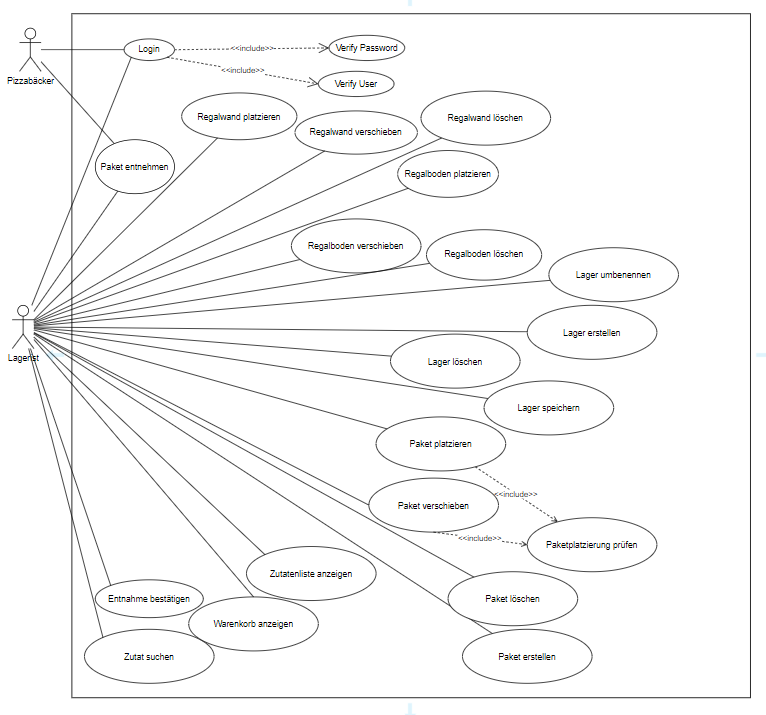
\includegraphics[width=17cm]{Bilder/Kapitel/use-case-diagramm}
	\caption{Use-Case-Diagramm}
	\label{fig:Use-Case-Diagramm}
\end{figure}


\subsection{Anwendungsfälle}

\subsubsection{Regalwand löschen}
\textbf{Titel:} Regalwand löschen\\
\textbf{Autor:} Artur Konkel\\
\textbf{Akteure:} Lagerist\\
\textbf{Fachlicher Auslöser:} Regalwand soll entfernt werden\\
\textbf{Vorbedingungen:} Der Lagerist ist mit seinem Benutzeraccount im Lagersystem angemeldet sein; es wurde bereits ein Lager erstellt, dieses wurde ausgewählt im Bearbeitungsmodus\\
\textbf{Standardablauf:}
\begin{enumerate}
	\item Lagerist: Auswahl der Regalwand, die zu löschen ist
	\item Lagerist: löschen der Regalwand
	\item System: Prüfung, ob Regalwand ohne Konflikte zu löschen ist
	\item System: Prüfung OK. Löschen der Regalwand
\end{enumerate}\\
\textbf{Alternative Abläufe / Fehlersituationen / Sonderfälle:}
\begin{itemize}
	\item 4a System: Das Löschen der Regalwand ist nicht möglich, da dann Regalböden in der Luft liegen würden
	\subitem 4a1 System: Benachrichtigung an Lagerist
	\subitem 4a2 Lagerist bestätigt Benachrichtigung
	\item 4b System: Das löschen der Regalwand ist nicht möglich, da noch Pakete auf einem Regalboden liegen,
	welcher dann in der Luft liegen würde
	\subitem 4b1 System: Benachrichtigung an Lagerist
	\subitem 4b2 System: Lagerist bestätigt Benachrichtigung

\end{itemize}
\textbf{Nachbedingung / Ergebnis:} Regalwand wurde dem Lager entfernt\\
\textbf{Nicht-funktionale Anforderungen:} Sprechende Fehlermeldung\\
\textbf{Parametrisierbarkeit / Flexibilität:} - \\
\textbf{Nutzungshäufigkeit / Mengengerüst:} wöchentlich\\

\subsubsection{Regalboden platzieren}
\textbf{Titel:} Regalboden platzieren\\
\textbf{Autor:} Artur Konkel\\
\textbf{Akteure:} Lagerist\\
\textbf{Fachlicher Auslöser:} Regal soll mit einem zusätzlichen Regalboden erweitert werden\\
\textbf{Vorbedingungen:} Der Lagerist ist mit seinem Benutzeraccount im Lagersystem angemeldet sein; es wurde
bereits ein Lager erstellt, dieses wurde ausgewählt im Bearbeitungsmodus. Regalboden kann nur zwischen zwei
Regalwänden platziert werden.\\
\textbf{Standardablauf:}
\begin{enumerate}
	\item Lagerist: platziert Regalboden an gewünschter Stelle
	\item System: Prüft, ob Stelle valide
	\item System: Prüfung erfolgreich. Platzierung des Regalbodens an gewünschter Stelle
\end{enumerate}\\
\textbf{Alternative Abläufe / Fehlersituationen / Sonderfälle:}
\begin{itemize}
	\item 3a System: Prüfung fehlgeschlagen. Hinweis an Nutzer, dass Platzierung an gewünschter Stelle nicht möglich ist
	\subitem 3a1: Lagerist bestätigt Meldung
\end{itemize}
\textbf{Nachbedingung / Ergebnis:} Regalboden wurde im Lager platziert\\
\textbf{Nicht-funktionale Anforderungen:} - \\
\textbf{Parametrisierbarkeit / Flexibilität:} - \\
\textbf{Nutzungshäufigkeit / Mengengerüst:} wöchentlich\\

\subsubsection{Paket erstellen}
\textbf{Titel:} Neue Zutatenpakete ins Lagersystem eingeben\\
\textbf{Autor:} Anna-Livia Martin\\
\textbf{Akteure:} Lagerist\\
\textbf{Fachlicher Auslöser:} Neue Zutaten vom Lieferanten sind angekommen und müssen ins System eingepflegt werden\\
\textbf{Vorbedingungen:} Login erfolgreich, Lager erstellt\\
\textbf{Standardablauf:}\\
\begin{enumerate}
    \item Lagerist: Zutat auswählen
    \item Lagerist: Größe auswählen
    \item Lagerist: bestätigt Angaben
    \item System: erstellt Paket
\end{enumerate}\\
\textbf{Alternative Abläufe / Fehlersituationen / Sonderfälle:}\\
\begin{itemize}
	\item 1a die Zutat ist noch nicht vorhanden
		\subitem 1a1 neue Zutat erstellen
		\subitem 1a2 System zeigt neue Zutat an
		\subitem 1a3 weiter bei 2
	\item 2a benötigte Größe nicht vorhanden
		\subitem 2a1 Lagerist erstellt individuelle Größe
		\subitem 2a2 Lagerist speichert Größe
		\subitem 2a3 weiter bei 2
\end{itemize}
\textbf{Nachbedingung/Ergebnis:} Das neue Zutatenpaket ist erstellt, muss aber noch platziert werden\\
\textbf{Nicht-funktionale Anforderungen:} Validitätsüberprüfung der Paketinformationen < zwei sec.\\
\textbf{Parametrisierbarkeit / Flexibilität:} Informationen der Pakete importierbar\\
\textbf{Nutzungshäufigkeit / Mengengerüst:} alle zwei Tage\\

\subsubsection{Neue Zutatenpakete platzieren}
\textbf{Titel:} Neue Zutatenpakete platzieren\\
\textbf{Akteure:} Lagerist\\
\textbf{Autor:} Anna-Livia Martin\\
\textbf{Fachlicher Auslöser:} Es wurde ein neues Zutatenpaket erstellt, welches noch im Lager platziert werden muss, das Paket ist noch nicht platziert\\
\textbf{Vorbedingungen:} Login erfolgreich, Lager erstellt, Neue Zutatenpakete erstellt und liegen im "noch zu platzieren" Teil der Software\\
\textbf{Standardablauf:}
\begin{enumerate}
    \item Lagerist: platziert die Pakete manuell\\
    \item System: überprüft in unter einer Sekunde pro Paketplatzierung, ob das Paket an dieser Stelle platzierbar ist oder nicht\\
	\item System: platziert Paket\\
\end{enumerate}
\textbf{Alternative Abläufe / Fehlersituationen / Sonderfälle:}
\begin{itemize}
	\item 2a System stellt fest, dass sich das Paket nicht dort platzieren lässt, wo der Lagerist es haben möchte, da nicht genug Platz ist
		\subitem 2a1 System zeigt an, dass man dort nichts platzieren kann
		\subitem 2a2 weiter bei 1
	\item 2b System stellt fest, dass sich das Paket nicht dort platzieren lässt, wo der Lagerist es haben möchte, da das Paket zu schwer ist
		\subitem 2b1 System zeigt an, dass das Paket zu schwer ist für die Ablagefläche
		\subitem 2b2 weiter bei 1
	\item 2c System stellt fest, dass sich das Paket nicht dort platzieren lässt, wo der Lagerist es haben möchte, da es Lebensmittelunverträglichkeiten mit diesem Paket gibt
		\subitem 2c1 System zeigt an, dass man dort nichts platzieren kann, aufgrund von Lebensmittelunverträglichkeiten
		\subitem 2c2 weiter bei 1
	\item 2d System stellt fest, dass sich das Paket nicht dort platzieren lasst, wo der Lagerist es haben möchte, da das darunterliegende Paket nicht tragfähig genug ist
		\subitem 2d1 System zeigt an, dass man dort nicht platzieren kann, da das darunterliegende Paket nicht tragfähig genug ist
		\subitem 2d2 weiter bei 1\\
\end{itemize}
\textbf{Nachbedingung/Ergebnis:}  Die neuen Zutatenpakete sind erfolgreich ordnungsgemäß platziert worden\\
\textbf{Nicht-funktionale Anforderungen:} Reaktionszeit bei Paketplatzierungsüberprüfung < eine Sekunde\\
\textbf{Parametrisierbarkeit / Flexibilität:} falsch platzierbare Pakete lassen sich erneut platzieren\\
\textbf{Nutzungshäufigkeit / Mengengerüst:} alle zwei Tage\\

\subsubsection{Paket im Lagersystem verschieben}
\textbf{Titel:} Paket im Lagersystem verschieben\\
\textbf{Autor:} Sarah Schwarzer\\
\textbf{Akteure:} Lagerist\\
\textbf{Fachlicher Auslöser:} Zutatenpaket muss im Lager umplatziert werden, um Platz für neue Lieferungen zu schaffen oder um eine effizientere Struktur im Lager zu gewährleisten\\
\textbf{Vorbedingungen:} erfolgreicher Login und es gibt bereits bestehendes Pakete im Lager, welches schon platziert wurde und das Lager selbst existiert schon\\
\textbf{Standardablauf:}
\begin{enumerate}
    \item Lagerist: öffnet Lagersystem und wählt jeweiligen Bereich für die manuellen Änderungen aus\\
    \item Lagerist: identifiziert die Pakete, welche umplatziert werden sollen und wählt diese aus\\
    \item Lagerist: fügt die ausgewählten Pakete an der gewünschten Position ein\\
    \item System: überprüft, ob die ausgewählte Position passt, um Konflikte mit anderen Paketen zu vermeiden oder Probleme bei der Lagerplatzierung \\
    \item System: aktualisiert den Lagerbestand und die Lagerplatzierung automatisch\\
\end{enumerate}
\textbf{Alternative Abläufe / Fehlersituationen / Sonderfälle:}
\begin{itemize}
	\item 4a System stellt fest, dass ausgewählte Position im Lager nicht geeignet ist (z.B. Größe, Tragfähigkeit)
		\subitem 4a1 System markiert nicht funktionierende Positionen und schlägt alternative Standorte vor
		\subitem 4a2 Lagerist wählt daraufhin alternative Position aus
		\subitem 4a3 weiter bei 3\\
\end{itemize}
\textbf{Nachbedingung / Ergebnis:} Pakete wurden erfolgreich an den gewünschten Ort verschoben, Lagerbestand und Lagerplatzierung wurden aktualisiert\\
\textbf{Nicht-funktionale Anforderungen:} Umlagerung von Paketen soll innerhalb von fünf Sekunden abgeschlossen sein\\
\textbf{Parametrisierbarkeit / Flexibilität:} es können flexibel Pakete umplatziert werden, falls es zu ändernde Anforderungen gibt\\
\textbf{Nutzungshäufigkeit / Mengengerüst:} je nach Bedarf, alle zwei Tage

\subsubsection{Lager im System umbenennen}
\textbf{Titel:} Lager im System umbenennen\\
\textbf{Autor:} Sarah Schwarzer\\
\textbf{Akteure:} Lagerist\\
\textbf{Fachlicher Auslöser:} die Bezeichnung/der Name eines Lagers muss geändert werden, damit eine gute Übersichtlichkeit und Organisation gewährleistet werden kann\\
\textbf{Vorbedingungen:} erfolgreicher Login und es gibt bestehende Lager, die vom System bereits erfasst wurden\\
\textbf{Standardablauf:}
\begin{enumerate}
    \item Lagerist: öffnet Lagersystem, loggt sich ein und gelangt automatisch zur Übersicht, wo alle Lager aufgelistet sind die existieren\\
    \item Lagerist: wählt das zu ändernde Lager aus der Übersicht aus\\
    \item System: öffnet Eingabefeld für die Änderung\\
    \item Lagerist: gibt neuen Namen ein und bestätigt die Eingabe\\
    \item System: überprüft, dass die Eingabe nicht leer ist\\
    \item System: speichert den neuen Lagernamen und aktualisiert die Anzeige\\
\end{enumerate}
\textbf{Alternative Abläufe / Fehlersituationen / Sonderfälle:}
\begin{itemize}
	\item 5a System stellt fest, dass Lagername nicht verfügbar ist
		\subitem 5a1 System informiert den Lageristen, dass der Name bereits existiert
		\subitem 5a2 Lagerist gibt erneut einen Namen ein und bestätigt
		\subitem 5a3 weiter bei 6\\
\end{itemize}
\textbf{Nachbedingung / Ergebnis:} Pakete wurden erfolgreich an den gewünschten Ort verschoben, Lagerbestand und Lagerplatzierung wurden aktualisiert\\
\textbf{Nicht-funktionale Anforderungen:} Umlagerung von Paketen soll innerhalb von einer Sekunde abgeschlossen sein\\
\textbf{Parametrisierbarkeit / Flexibilität:} es können flexibel Pakete umplatziert werden, falls es zu ändernde Anforderungen gibt\\
\textbf{Nutzungshäufigkeit / Mengengerüst:} je nach Bedarf, alle zwei Tage

\subsubsection{Zutatenpakete aus dem Lager entnehmen}
\textbf{Titel:} Zutatenpakete aus dem Lager entnehmen\\
\textbf{Autor:} Vivien Weber\\
\textbf{Akteure:} Pizzabäcker, Lagerist\\
\textbf{Fachlicher Auslöser:} Zutatenpakete müssen aus dem Lager entnommen werden für den täglichen Bedarf\\
\textbf{Vorbedingungen:}
\begin{enumerate}
	\item Lagerist ist mit seinem Benutzeraccount im Lagersystem angemeldet
	\item Die benötigten Mengen an Zutatenpaketen sind im Lagersystem enthalten und werden angezeigt
\end{enumerate}\\
\textbf{Standardablauf:}
\begin{enumerate}
	\item Lagerist: Öffnet im System das gewünschte Lager zur Entnahme
	\item Lagerist: Sucht nach der gewünschten Zutat oder wählt sie in der Zutaten-Ansicht aus
	\item System: Sucht in weniger als fünf Sekunden nach den genauen Positionen der benötigten Pakete und markiert diese auf dem Bildschirm
	\item Lagerist: Fügt die passenden, markierten Zutatenpakete dem Warenkorb hinzu
	\item Lagerist: Überprüft die Vollständigkeit der benötigten Zutatenpakete im Warenkorb
	\item Lagerist: Hat die Möglichkeit, die Entnahme zu bestätigen oder abzubrechen
	\item Lagerist: Bestätigt die Entnahme
	\item System: Zeigt erfolgreichen Abschluss des Vorgangs an
\end{enumerate}\\
\textbf{Alternative Abläufe / Fehlersituationen / Sonderfälle:}
\begin{enumerate}
	\item 2a Falls die benötigten Zutaten nicht im Lager vorhanden sind, erhält der Lagerist eine Benachrichtigung und muss entsprechende Maßnahmen ergreifen (z.B. Nachbestellung)
	\subitem 2a1 Lagerist erhält eine Benachrichtigung über fehlende Zutaten im Lager
	\subitem 2a2 weiter bei 1
	\item 4a Falls ein zu entnehmendes Paket unter einem/mehreren nicht benötigten Paket/en liegt, werden die nicht benötigten Pakete neu platziert
	\subitem 4a2 System platziert die oberen Pakete an der Stelle des entnommenen Pakets
	\subitem 4a3 weiter bei 6
\end{enumerate}\\
\textbf{Nachbedingung / Ergebnis:} Die benötigten Zutatenpakete wurden erfolgreich aus dem Lager entnommen und dem Pizzabäcker übergeben.\\
\textbf{Nicht-funktionale Anforderungen:} Die Ausgabe der Zutatenpaket-Positionen erfolgt in weniger als fünf Sekunden.\\
\textbf{Parametrisierbarkeit / Flexibilität:} Das System kann an verschiedene Mengenbedarfe und Lagerkonfigurationen angepasst werden.\\
\textbf{Nutzungshäufigkeit / Mengengerüst:} einmal täglich

\subsubsection{Zutatenpaket löschen}
\label{Zutatenpakete_entnehmen}
\textbf{Titel:} Zutatenpaket aus dem Regal löschen\\
\textbf{Autor:} Vivien Weber\\
\textbf{Akteure:} Lagerist\\
\textbf{Fachlicher Auslöser:} Lagerist hat ein falsches Paket erstellt und muss es wieder löschen\\
\textbf{Vorbedingungen:}
\begin{enumerate}
	\item Lagerist ist mit seinem Benutzeraccount im Lagersystem angemeldet
	\item Lagerist befindet sich in der Lager-Ansicht "Platzieren"
\end{enumerate}\\
\textbf{Standardablauf:}
\begin{enumerate}
	\item Lagerist: wählt ein Paket aus, das gelöscht werden soll
	\item System: prüft, ob sich auf diesem Paket noch weitere Pakete befinden
	\item Lagerist: bestätigt das Löschen des ausgewählten Pakets
	\item Das System zeigt einen erfolgreichen Abschluss des Vorgangs an
\end{enumerate}\\
\textbf{Alternative Abläufe / Fehlersituationen / Sonderfälle:}
\begin{enumerate}
	\item 2a Falls das zu löschende Paket unter einem/mehreren Paket/en liegt, werden diese neu platziert
	\subitem 2a2 System platziert die oberen Pakete an der Stelle des entnommenen Pakets
	\subitem 2a3 weiter bei 3
\end{enumerate}\\
\textbf{Nachbedingung / Ergebnis:} Ein Zutatenpaket wird erfolgreich aus dem Regal gelöscht\\
\textbf{Nicht-funktionale Anforderungen:} -\\
\textbf{Parametrisierbarkeit / Flexibilität:} -\\
\textbf{Nutzungshäufigkeit / Mengengerüst:} Dieser Anwendungsfall tritt bei Bedarf auf, wenn ein Paket gelöscht werden muss.\\

\section{"Gegenstandwelt" des Systems / Datenmodell (Domänenmodell)}
\label{sec:domaenenmodell}
Es gibt insgesamt zwei verschiedene Rollen, den Pizzabäcker und den Lageristen. Beide sind Benutzer mit Namen, Passwort,
Rolle, Probilbild und benutzerId. Jeder Benutzer hat einen Warenkorb. Außerdem kann er unbegrenzt viele Zutatenpakete
entnehmen und dort platzieren. Ein Zutatenpaket besteht aus einer Zutat und einem Paket. Eine Zutat hat einen Namen,
Unverträglichkeiten und ein Icon. Ein Paket haben eine Breite, Höhe, Gewicht, Tragfähigkeit. Jedes Zutatenpaket
gehört in ein Lager, wobei ein Lager mehrere Zutatenpakete haben kann. Jedes Lager hat dabei einen Namen und eine
eindeutige ID. Dieses kann aus mehreren Regalen bestehen, welche aus Regalwänden und Regalböden zusammengesetzt
sind. Diese haben jeweils ebenso eine Höhe und eine Breite. Es gibt immer
mindestens zwei Regalwände und mindestens einen Regalboden pro Regal. Ein Regal hat mindestens ein Ablagebereich mit einer
Höhe und Breite. Regale haben mindestens einen Ablagebreich, definiert durch Regalwände und Regalböden.\\

\begin{figure}[H]
	\centering
	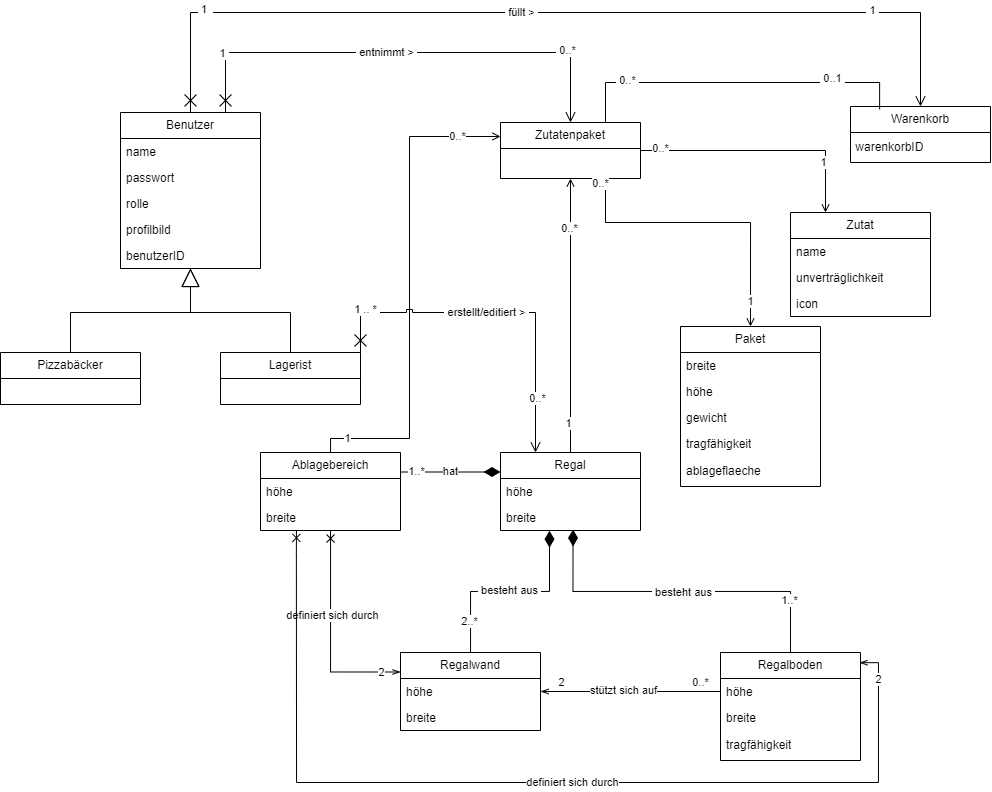
\includegraphics[width=\textwidth]{Bilder/Kapitel/domaenenmodell}
	\caption{Domänenmodell}
	\label{fig:domaenenmodell}
\end{figure}

\section{Styleguide}
\subsection{Einführung}
Dieser Styleguide soll ein durchgängiges und professionelles Erscheinungsbild der Software sicher stellen.
Er bietet ausführliche Vorgaben der Gestaltung, die Designern, Entwicklern und Testern als Orientierung dienen sollen.
Eine konsistente Benutzererfahrung wird geschaffen, die sowohl ansprechend als auch benutzerfreundlich ist.
Von der Farbpalette und Typografie bis hin zu Layouts und Navigationselementen, sind alle Aspekte des Designs und der Benutzerinteraktion aufgelistet.
Dieser Guide dient als Grundlage für alle, die an der Entwicklung und stetigen Verbesserung der Software beteiligt sind und ist verbindlich.

\subsection{Inhalt}
Der Styleguide ist in folgende Punkte untergliedert:

\begin{itemize}
    \item Gestaltungsvorgaben
    \item UI-Komponenten
    \item Interaktionsdesign
    \item Entwicklungsvorgaben
    \item Dokumentation
    \item Wartung und Updates
\end{itemize}

\subsection{Gestaltungsvorgaben}
Die gewählten Farbschemata setzen sich aus primären Beigetönen, sowie kräftigen Rot- und Grüntönen als Sekundärfarben zusammen.
Diese Farben sollen den Pizza-Flair für die Software widerspiegeln. Schwarz, Weiß und Braun sind als Akzentfarben eingesetzt.
Diese Kombination schafft eine harmonische Farbpalette, die modern und klassisch wirkt.\\
\\
In der Typografie wird auf die Schriftart Arial als primäre Schriftart gesetzt. Ergänzt wird diese mit der Schriftart AkayaTelivigala,
welche hauptsächlich für den Titel verwendet wird. Die festgelegten Schriftgrößen sorgen für eine gute Übersicht und Lesbarkeit im Zusammenhang mit den Schriftarten.\\
Das Layout berücksichtigt harmonische Abstände zwischen den Elementen sowie zwischen Elementen und Überschriften.
Die Abstände variieren, um eine ästhetische Gestaltung zu ermöglichen. Margin und Padding werden ebenfalls flexibel gehandhabt,
um eine ansprechende Benutzeroberfläche zu gewährleisten.\\
\\
Icons und Bilder werden in PNG-Format dargestellt, damit die Elemente klar und hochwertig erscheinen.

\paragraph{Farbschemata}
Primärfarben: \#DCCFC4 (Beige) mit 100\% und 50\% Deckkraft\\
Sekundärfarben: \#BC1818 (Rot), \#49AD33 (Grün)\\
Akzentfarben: \#000000 (Schwarz), \#FFFFFF (Weiß), \#74442D (Braun) mit 70\% Deckkraft

\paragraph{Typografie}
\subparagraph{Schriftarten}
Primäre Schriftart: Arial, sans serif\\
Sekundäre Schriftart: AkayaTelivigala, handwritten

\subparagraph{Schriftgrößen}
Titel: 52px\\
Untertitel: 23px\\
Fließtext: 12px\\
Kleintext: 6px

\paragraph{Layout}
\subparagraph{Abstände}
Zwischen Elementen: unterschiedlich, wird entsprechend angepasst\\
Zwischen Elementen und Überschriften: 20px, 90px, 31px, unterschiedlich, wird entsprechend angepasst

\subparagraph{Margin und Padding}
Außenabstände: unterschiedlich, wird entsprechend angepasst\\
Innenabstände: unterschiedlich, wird entsprechend angepasst

\subsubsection*{Icons und Bilder}
Icons: PNG, maximal 24px x 24px\\
Bilder: PNG, maximale Breite 800px

\subsection{UI-Komponenten}
Buttons sind entscheidend für die Benutzerinteraktion und sollen klar und einladend gestaltet sein.
Sie erhalten alle einen leichten Schein nach außen in unterschiedlichen Farben, der betont, dass sie interaktiv sind.\\
\\
Die Eingabefelder sind ein zentrales Element der Benutzerinteraktion und tragen zum Wesentlichen zu der Benutzerfreundlichkeit bei.\\
\\
Die Navigation in der horizontalen Ebene sind bedeutend, um den Benutzern eine effiziente Navigation durch die Software zu ermöglichen.\\
\\
Das Burger-Menü bietet eine kompakte und leicht zugängliche Möglichkeit Navigationselemente darzustellen, wenn der Platz begrenzt ist.
Die drei horizontalen Linien sind ein gängiges Symbol für solche Anwendungen, das die meisten Benutzer sofort erkennen und verstehen.\\
\\
Die Liste strukturiert die Informationen und hilft, Daten schnell zu erfassen und einzusetzen.

\paragraph{Buttons}
\subparagraph{Stile}
Primär: Hintergrund: \#C3E0C2 (Hellgrün) \#F0C8C9 (Hellrot), Text: \#BC1818 (Rot) \#49AD33 (Grün), Rahmen: solid 1px \#BC1818 (Rot), \#49AD33 (Grün)\\
Sekundär: Hintergrund: \#FFFFFF (Weiß), Icon: \#000000 (Schwarz) \#FFFFFF (Weiß) \#49AD33 (Grün) (für Buttons hauptsächlich in der Navigationsleiste,
aber auch in dem restlichen Programm)

\subparagraph{Zustände}
Standard: Opazität 100\%\\
Hover: alle haben Schein nach außen \#3FA535, \#CD1719 (für wichtige Button), \#FFFFFF (Weiß)(für Navigationsbutton)\\
Deaktiviert: sieht aus wie gehabt

\paragraph{Formulare}
\subparagraph{Eingabefelder}
Primär: Hintergrund \#C3E0C2 (Pastellgrün)\\
Text: \#49AD33 (Grün)\\
Rahmen: 1px solid \#49AD33 (Grün)\\
Fokus: Schein nach außen \#3FA535 (Grün), Text verschwindet, Text-Cursor erscheint\\
Fehler: Hintergrund \#F0C8C9, Rahmen 1px solid \#BD181E

\paragraph{Navigationselemente}
\subparagraph{Horizontale Ebene}
Abstand: 16px zwischen den Buttons\\
Stil: Buttons sollen in einer horizontalen Ebene angezeigt werden\\
Hover: Schein nach außen \#FFFFFF (Weiß)

\subparagraph{Burger-Menü}
Verwendung: wird verwendet, um Platz zu sparen und die Benutzerfreundlichkeit der Software zu verbessern\\
Darstellung: rundes Icon mit drei horizontalen Linien, Größe 10px x 10px, Farbe \#FFFFFF (Weiß) \#49AD33 (Grün)\\
Abstand: 16px Abstand zu anderen Elementen\\
Platzierung: Rechts oben in der Navigationsleiste und rechts in der Ecke von ausgewählten Icons\\
Interaktion: bei Klick öffnet sich Pop-Up/vertikales Menü\\
Animation: Weiches Ein- und Ausblenden des Pop-Ups innerhalb von 0,3 Sekunden

\paragraph{Tabellen und Listen}
Art Liste: keine Aufzählungszeichen, drei Elemente pro Zeile, rechts Leiste zum Bewegen in der Liste\\
Abstand: 16px zwischen den Elementen

\subsection{Interaktionsdesign}
Die Gestaltung von Animationen und Übergängen ermöglichen es, dem Nutzer eine flüssige und ansprechende Benutzererfahrung zu versichern.

\paragraph{Animation und Übergänge}
Übergänge: 0,3 Sekunden Ease-In-Out für Hover Effekte\\
Techniken: Drag \& Drop\\
Feedback: wenn Element an ungültige Position gezogen wird

\subsection{Dokumentation}
Für eine einheitliche Dokumentation innerhalb des Projekts wurden Standards festgelegt, die in LaTeX verfasst sind.
Es ist sinnvoll für technisch anspruchsvolle und ausführliche Dokumentationen. Denn diese Dokumentationen wirken dadurch qualitativ und konsistent.
Das Ganze erleichtert das Verständnis für alle Nutzer und fördert die Weiterentwicklung des Projekts.

\paragraph{Dokumentationsstandards}
Format: LaTeX

\subsection{Wartung und Updates}
Dieser Prozess stellt sicher, dass alle Anpassungen sorgfältig geprüft und abgestimmt werden, bevor sie implementiert werden.
Durch diesen Ansatz wird sicher gestellt, dass der Styleguide nicht nur aktuell bleibt, sondern auch auf die Erfahrungen der Nutzer eingeht.

\paragraph{Änderungen}
Prozess: Änderungen am Styleguide müssen durch das Team genehmigt werden, Anträge für Veränderungen per Pull-Request\\
Häufigkeit: Halbjährliche Überprüfung

\paragraph{Feedback}
Methoden: regelmäßige Umfragen\\
Aufnahme: Rückmeldungen in den Styleguide einfließen lassen

\section{Benutzerführung für die Anwendung}
\label{sec:benutzerfuehrung}
Um die Anwendung zu nutzen, schalten Sie zunächst Ihren Computer ein und öffnen die Anwendung.

\subsection{Anmeldung/Login}
Sie sehen den Namen Ihrer Pizzeria auf dem Bildschirm. Wenn Sie bereits über einen User-Account mit einem Username
und Passwort verfügen, können Sie sich mit Ihren Daten einloggen. Geben Sie Ihren Usernamen und Ihr Passwort ein,
um sich anzumelden.

\subsection{Startseite}
Nach der Anmeldung befinden Sie sich auf der Startseite. Oben rechts können Sie auf Ihr Profil zugreifen. Oben links
haben Sie die Möglichkeit, die Anwendung mit ``X'' zu schließen oder mit ``-'' zu minimieren. Auf der Startseite
stehen Ihnen verschiedene Optionen zur Verfügung:

\begin{itemize}
	\item Sie können direkt auf das gewünschte Lager klicken, um zum Lagerentnahme-Screen zu gelangen.
	\item Sie können ein Lager mit einem Stern markieren, um es als Favorit hinzuzufügen.
	\item Mit dem ``+'' im noch nicht belegten Lager können Sie ein neues Lager erstellen.
	\item Über das Burgermenü oben rechts über einem gewünschten Lager können Sie:
	\begin{itemize}
		\item Zutatenpakete hinzufügen.
		\item Zutatenpakete verschieben.
		\item Das ausgewählte Lager im Editor öffnen, vorausgesetzt, es sind keine Zutatenpakete darin enthalten; andernfalls erscheint eine Fehlermeldung.
	\end{itemize}
\end{itemize}

\subsection{Lageransicht – Entnahme}
In der Entnahme-Ansicht sehen Sie oben mittig den Namen des Lagers und den Hinweis, dass Sie sich in der ``Entnahme''
befinden. In der Mitte des Bildschirms befindet sich die Regalansicht mit den vorhandenen Regalböden, -wänden und
Zutatenpaketen. Oben links können Sie die Anwendung mit ``X'' schließen oder mit ``-'' minimieren. Oben rechts
gelangen Sie auf Ihr Profil, daneben befindet sich ein Burgermenü mit den gleichen Optionen wie auf der Startseite:
Zutatenpakete verschieben und das ausgewählte Lager im Editor öffnen (unter der Bedingung, dass keine Zutaten-Pakete
darin enthalten sind, sonst Fehlermeldung). Unten finden Sie eine Leiste mit dem aktuellen Lager und anderen
bestehenden Lagern. Auch hier können Sie ein neues Lager erstellen.

Rechts gibt es zwei Bereiche:
\begin{itemize}
	\item \textit{Unten:} Der Warenkorb, in dem Sie überprüfen können, welche Zutatenpakete sich darin befinden. Sie können den Entnahme-Vorgang abschließen oder abbrechen.
	\item \textit{Oben:} Eine Such- und Auswahlfunktion für Zutatenpakete, mit der Sie nach dem Namen der gewünschten Zutat suchen oder nach bestimmten Eigenschaften filtern können. Sie können die gewünschte Zutat durch Klick auf das Icon und die Beschriftung auswählen.
\end{itemize}

In der Entnahme-Ansicht können Sie die gewünschten Zutatenpakete per Drag \& Drop in den Warenkorb ziehen.

\subsection{Lageransicht – Platzieren}
Die Platzieren-Ansicht ähnelt der Entnahme-Ansicht, unterscheidet sich jedoch darin, dass es rechts unten keinen
Warenkorb gibt. In der Mitte befindet sich die Regalansicht mit den vorhandenen Regalböden und -wänden sowie
gegebenenfalls bereits vorhandenen Zutatenpaketen. Oben mittig sehen Sie den Lagername und den Hinweis, dass Sie
sich in ``Platzieren'' befinden. Oben links können Sie die Anwendung mit ``X'' schließen oder mit ``-'' minimieren.
Oben rechts gelangen Sie auf Ihr Profil, daneben befindet sich ein Burgermenü mit den gleichen Optionen wie auf der Startseite.

Unten finden Sie eine Leiste mit dem aktuellen Lager und anderen bestehenden Lagern. Auch hier können Sie ein neues
Lager erstellen. Rechts gibt es zwei Bereiche:
\begin{itemize}
	\item \textit{Oben:} Die Such- und Auswahlfunktion für Zutatenpakete. Sie können nach dem Namen der gewünschten Zutat suchen, nach bestimmten Eigenschaften filtern, die gewünschte Zutat durch Klick auf das Icon und die Beschriftung auswählen und neue Zutaten mit dem ``+'' hinzufügen.
	\item \textit{Unten:} Bei Auswahl einer Zutat erscheinen die verfügbaren Maße des Pakets und die Anzahl, wie viele der Zutat in das Paket passen. Sie können auch ein Paket mit individuellen Maßen anlegen und die Auswahl mit den Buttons darunter bestätigen oder abbrechen.
\end{itemize}

In der Platzieren-Ansicht können Sie die gewünschten Zutatenpakete per Drag \& Drop ins Regal ziehen. Das System
überprüft dann die Größe, das Gewicht und mögliche Unverträglichkeiten der Pakete, um eine korrekte Platzierung sicherzustellen.

\subsection{Lagereditor}
Im Lagereditor sehen Sie oben mittig den Titel ``Lager-Editor''. Oben links können Sie die Anwendung mit ``X''
schließen oder mit ``-'' minimieren. Oben rechts gelangen Sie auf Ihr Profil. In der Mitte sehen Sie zunächst ein
leeres Regal, in das Sie Böden und Wände hinzufügen können. Diese können Sie nach Eingabe der gewünschten Maße in der
Regalansicht einfügen und verschieben. Unten finden Sie eine Leiste mit dem aktuellen Lager und anderen bestehenden
Lagern sowie die Möglichkeit, ein neues Lager zu erstellen. Rechts unten befinden sich zwei Buttons: Speichern und Löschen.

\section{Wireframes}
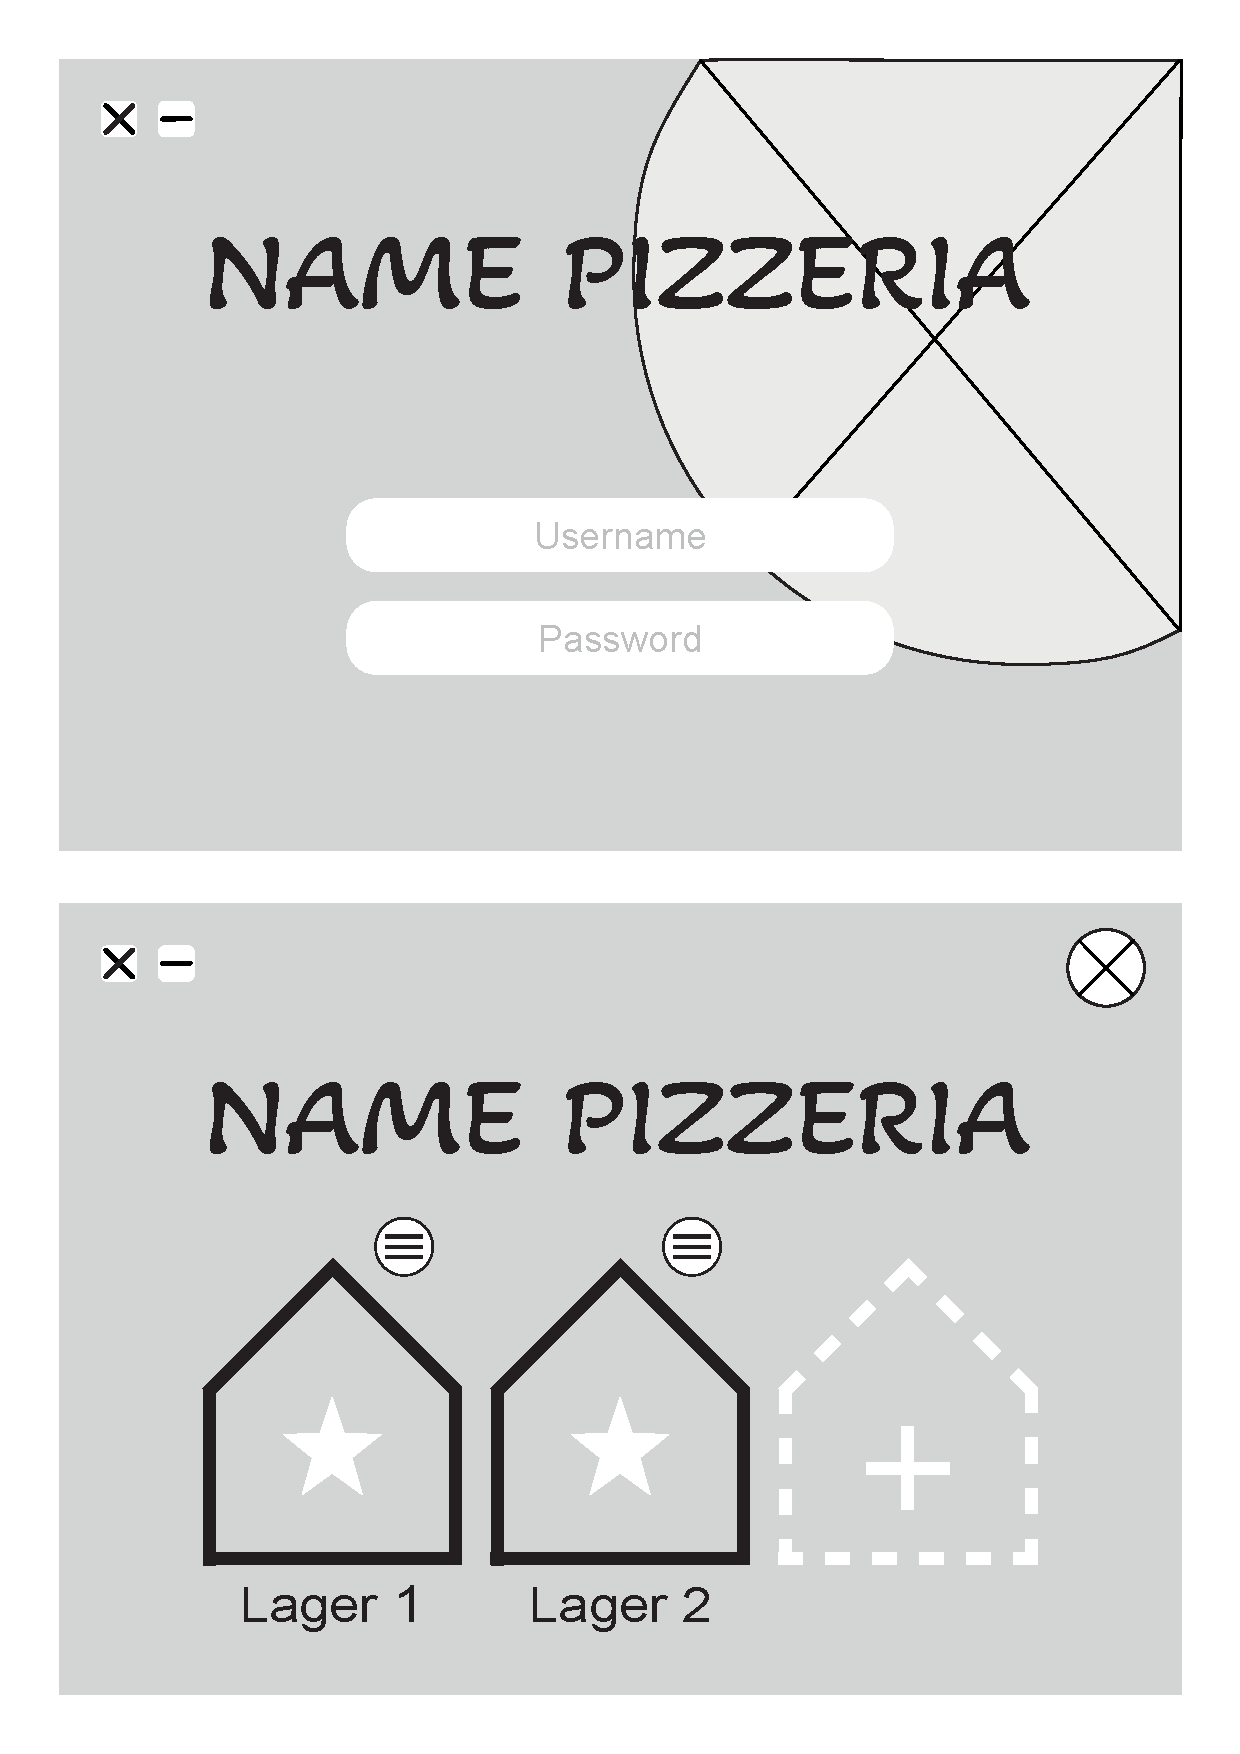
\includepdf[page=-]{Bilder/Kapitel/Wireframes_SWT}

% Ende der Datei
